\section{OpenCL based BFS optimization} \label{sec:bfs-opt}
In this section, we elaborate the OpenCL based BFS optimizations
on top of the pipelined structure. Particularly, we will focus on the 
memory access optimizations based on our pipeline design.
%which are critical to improve the BFS performance as discussed in Section \ref{sec:motivation}. 

%\subsection{Irregularity in BFS}
%\subsubsection{Irregular memory access}
%The basic BFS structure as mentioned in Figure \ref{fig:base-bfs} is well pipelined, 
%but it involves a large number of random memory accesses as analyzed 
%in \cite{Merrill2012scalable}. In the second stage, the vertex indices in the frontier 
%are usually not continuous, so the RPA read becomes random. For vertices with 
%larger degree, the CIA read can be considered as sequential memory access. Nevertheless, 
%the vertex degree of the graphs especially the social network follows the power-law 
%distribution and it indicates that there are a great number of low-degree vertices 
%and short sequential memory accesses. Particularly, since the vertex degree in 
%the BFS accelerator is known at run-time, the CIA read is usually aligned to the vertex 
%index data width (32 bits in this work). 
%
%In the third stage, when the status array 
%is located in the main memory, the status read is also random. When the vertex is un-visited, 
%random write is also required. In the last stage, frontier vertices typically write 
%sequentially because only part of the frontier neighbors become new frontiers 
%in the next BFS iteration, it is also random memory access by default. 
%While the frontier vertices are usually not sequential, the vertex level update 
%is also random. The massive random or short sequential
%memory accesses in combination result in the extremely low memory bandwidth utilization and 
%performance accordingly. 

%\subsubsection{Dependent data paths}

\subsection{Memory coalescing}
As analyzed in Section \ref{sec:motivation}, inefficient memory accesses 
are mainly caused by small data width, short burst accesses, and false 
dependent memory accesses. To be more specific, the data width of the 
sequential memory accesses ($CIA[idx]$) in $inspectFrontierCIA()$ are equal to that of 
the vertex index which is usually 32-bit in OpenCL, because the start address of the 
sequential memory access is not aligned in CSR. In addition, there are 
a large amount of low-degree vertices in realistic graphs. It indicates 
that many sequential memory accesses have very short burst size 
in $inspectFrontierCIA()$. Memory accesses with small data width and 
short burst also exist in $inspectFrontierRPA()$. They underutilize 
the memory bandwidth. False dependent memory accesses i.e. $level[v\_out]$ 
mainly appear in different iterations of $checkNgbVisitStatus()$. They 
also affect the memory access utilization dramatically. 

To improve the memory access efficiency with OpenCL, we try to coalesce the 
memory accesses with the following approaches.
First, we have both RPA and CIA arrays aligned.
For RPA array, the original RPA array is changed to the new sequence 
($RPA[0]$, $RPA[1]$ - $RPA[0]$), ($RPA[1]$, $RPA[2]$ - $RPA[1]$), ..., ($RPA[i]$, $RPA[i+1]$ - $RPA[i]$), ...
where $i$ is a vertex index. Given random request $RPA[i]$, the two 32-bit RPA read 
operations are combined to a single memory read aligned to 64-bit. For CIA array, it is typically read 
from $CIA[RPA[i]]$ to $CIA[RPA[i+1]$ sequentially when traversing the neighbors of vertex $i$. 
To ensure aligned neighbor traverse, we have both ends aligned to $B \times 32$-bit where $B$ refers to 
the number of batched data. Basically, $B$ vertices batched together can be read each time in $inspectFrontierCIA()$.
Note that additional padding i.e. '-1' may be added to ensure that CIA range of each vertex 
to be fully divided by $B$. With the data alignment and batching, the overall memory access efficiency 
improves despite the additional padding.

Secondly, $B$ neighbors must be processed in parallel in $checkNgbVisitStatus()$ to guarantee 
smooth pipelining, so $B$ also determines the number of parallel processing units i.e. 
$checkNgbVisitStatus()$. As $B$ neighbors are independent, it is natural to 
distribute them to the $B$ processing units. When the $B$ neighbors get processed 
in parallel, the false dependency is resolved accordingly. Nevertheless, 
$B$ parallel processing units of $checkNgbVisitStatus()$ may still 
be stalled due to the memory conflicts. Figure \ref{fig:write-conflict} 
shows the potential conflicts when checking the neighbors of a vertex in parallel.  
Both vertex 8 and Vertex 12 are neighbors of vertex 2 and they are supposed to be 
processed in parallel. However, $level[8]$ and $level[12]$ may stay in the same 
DRAM bank or on-chip buffer bank. As a result, they can only be processed sequentially.   

\begin{figure}
\center{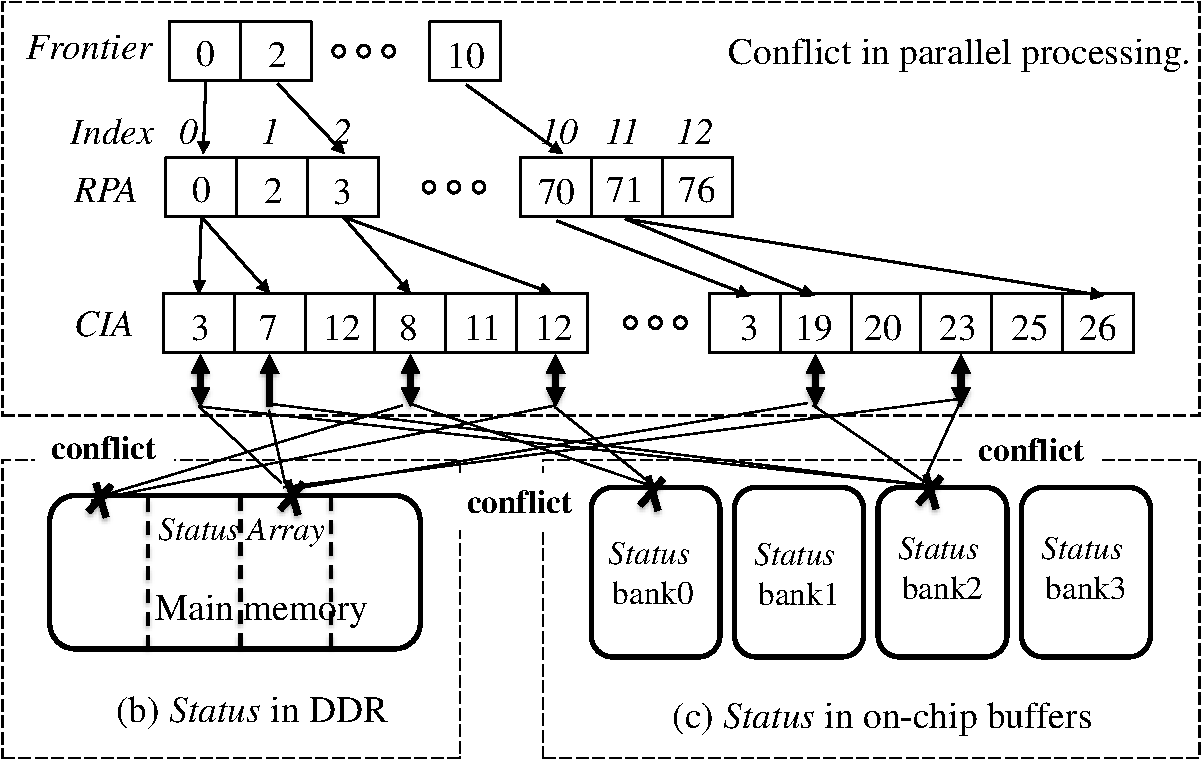
\includegraphics[width=0.7\linewidth]{write-conflict}}
    \caption{Conflicts among the parallel BFS data paths}
\label{fig:write-conflict}
\vspace{-1.2em}
\end{figure}

To resolve the above conflict, we propose the third approach. 
We reorder the outgoing neighbors of each 
vertex to ensure no conflict in the $B$ parallel update 
units. Algorithm \ref{alg:mem-coalescing} details the reordering 
together with the data alignment. The original CSR graph consists of
$RPA$ array and $CIA$ array and the reordered new CSR graph is stored 
in $newRPA$ array and $newCIA$ array respectively. The reordering roughly 
involves two steps. 1) Neighbors of each vertex are assigned to 
$B$ queues based on the modulo result of neighbor vertex index and $B$.
2) We get one data from each queue to construct a batch of $B$ data.
Repeat the process until all queues are empty. All the batched data 
are put into $newCIA$ array. '-1' will be used as padding to construct 
the batched data when the corresponding queue is empty earlier. 
$newRPA$ is updated accordingly to ensure the CSR storage format.

A typical example of the reordering and alignment is shown in Figure \ref{fig:graph-reorder}. 
In this example, batch size is 4. Vertex 0 has as 2 neighbors i.e. 
Vertex 3 and 7. They belong to the same bank i.e. Bank 3, because both mod(3,batch) 
and (7, batch) are equal to 3. Thus, six '-1' will be padded. While Vertex 11 
has five neighbors, they can be put into two batches and three '-1' need to 
be padded. Padding can vary and may bring in additional memory consumption. 
Larger batch size will incur more padding overhead but more parallel processing 
and higher memory bandwidth utilization can be expected.

With the data alignment, graph batching and reordering, memory accesses in 
$inspectFrontierRPA()$, $inspectFrontierCIA()$ and $checkNgbVisitStatus()$ 
are coalesced for parallel processing. Finally, note that graph reordering 
and data alignment need to be done only once and can be considered 
as graph pre-processing. The pre-processing can 
be done on general purposed processors. In fact, graph pre-processing is a 
common practice in many static graph processing systems \cite{Dai2017foregraph}
\cite{ham2016graphicionado} \cite{gui2019survey} \cite{shi2018graph} and 
the processing time is usually not the first-order concern.

\vspace{-0.5em}
\begin{algorithm}
	\caption{Data alignment and reordering of a CSR graph} \label{alg:mem-coalescing}
    \footnotesize
	\begin{algorithmic}[1]
		\State $queue[B]$
		\State $eid \gets 0$
		\For {$v \in V$}
		\State $newRPA[2v] \gets eid$
		\For {$(i \gets RPA[v]$ to $ RPA[v+1]$)}
		\State $j \gets mod(CIA[i],B)$
		\State $queue[j]$.write($CIA[i]$)
		\EndFor

		\State $D \gets 0$
		\While {(there are still non-empty queues in $queue[B]$)}
		\State $D \gets D + 1$
		\For{$(i \gets 0$ to $B)$}
		\State $eid \gets eid + 1$
		\If{($!queue[i].empty()$)} 
		\State {$newCIA[eid] \gets queue[i].read()$}
		\Else 
		\State {$newCIA[eid] \gets -1$}
		\EndIf
		\EndFor
		\EndWhile	
		\State $newRPA[2v + 1] \gets D \times B$
		\EndFor

	\end{algorithmic}
\end{algorithm}
\vspace{-0.5em}


\begin{figure}
\center{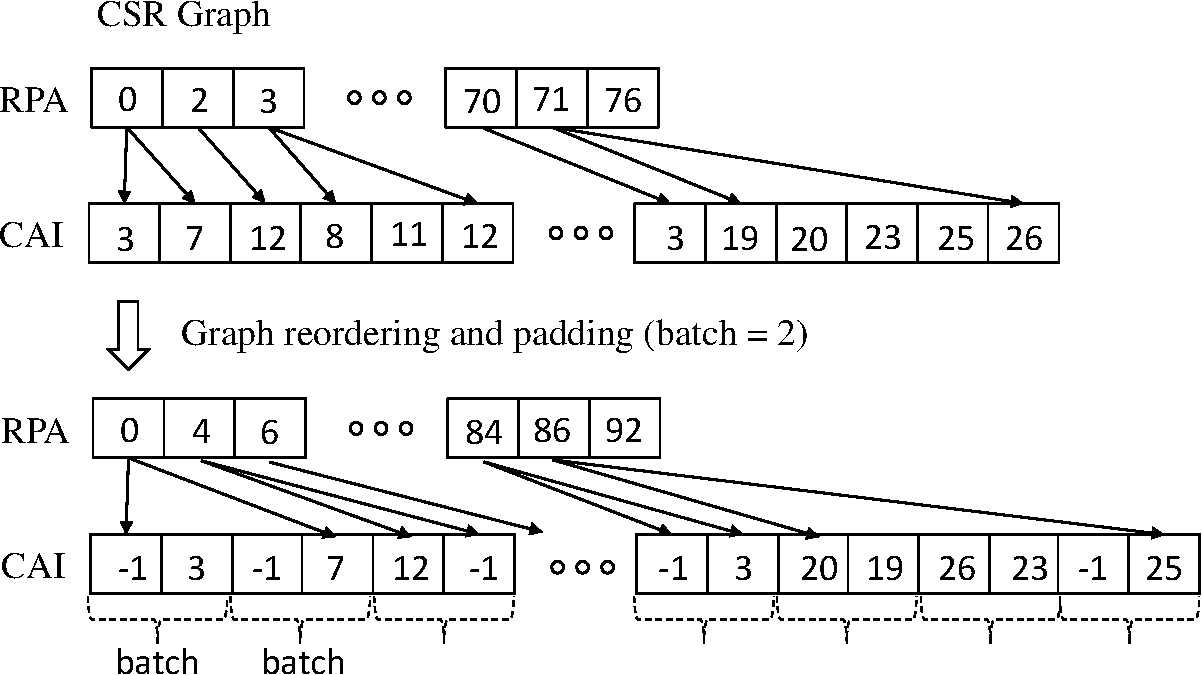
\includegraphics[width=0.82\linewidth]{graph-reorder}}
    \caption{CSR layout after the data alignment, graph reordering and batching}
\label{fig:graph-reorder}
\vspace{-1.5em}
\end{figure}

\subsection{On-chip bitmap buffering}
After the graph reordering and data alignment, there are still many random accesses
in $checkNgbVisitStatus()$ i.e. $level[v\_out]$. Although $B$ independent memory
access requests to DRAM can be issued in parallel, the random memory accesses
remain inefficient. Instead of using $level$ to determine the visiting status,
we utilize bitmap to represent the visiting status directly, which is also used in
some of the previous BFS accelerator designs \cite{gautier2016spector}.
Each vertex needs only one bit to determine whether it is visited.
The latest FPGAs with up to 500Mb on-chip buffer \cite{xilinxFPGA} can accommodate
graphs with 500 million vertices in theory, which fulfills the
requirements of many realistic graphs such as twitter2010
(42 million vertices) \cite{boldi2011layered}. It can be expected that
FPGAs with larger on-chip memory will be available in future,
This encourages us to have the whole bitmap stored in FPGA on-chip buffer.
Then the DRAM memory accesses in $checkNgbVisitStatus()$ can be replaced
with on-chip memory accesses, which guarantee determined
and low latency.

Meanwhile, we need to split the visiting status bitmap into $B$ banks
to fit the parallel processing of $checkNgbVisitStatus()$.
The visiting status of a vertex $v$ will be put into the $i$th memory
bank where $i = mod(id, B)$. The bitmap layout is consistent with the
graph reordering and batching. In addition, the processing unit
$checkNgbVisitStatus()$ needs to be changed and the new processing
is shown in Figure \ref{fig:bitmap}. Compared to the baseline BFS in
Algorithm \ref{alg:bfs}, the $level[v\_out]$ update is removed.
This will be explained in next subsection. While reading from or writing to the
on-chip buffer can be done in a single cycle and there is
write after read dependency in the new $checkNgbVisitStatus()$, the
initiation interval (II) of the kernel is 2.

In contrast, the authors \cite{ham2016graphicionado} proposed to use FIFOs
and crossbars to shuffle the data directly. When we implemented this scheme
with OpenCL, the II of the kernel goes up to 6, which is much larger than
the RTL designs. Basically, the number of outgoing neighbors vary for 
different frontier vertices, so OpenCL kernels are processing a stream 
with dynamic lengths. To pipeline the kernels, we need both a non-blocking control channel
and a data channel. When we implement the crossbar as well as FIFOs
with these channels, we must go through the control channels
for arbitration and then access the authorized data channels for data.
The arbitration and processing can hardly be parallelized in OpenCL directly
and incur long data dependency and large II.

\begin{figure}
\center{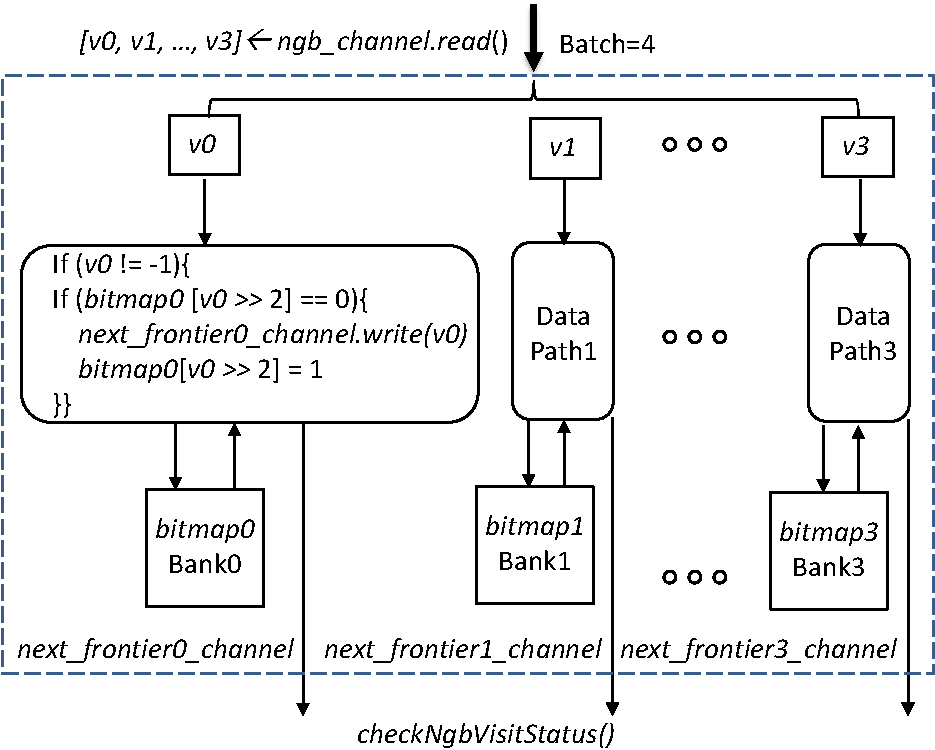
\includegraphics[width=0.72\linewidth]{bitmap}}
    \caption{Parallel processing with on-chip bitmap buffer}
\label{fig:bitmap}
\vspace{-1.2em}
\end{figure}

%\subsubsection{CPU assisted data reorganization}
%As discussed in Section \ref{sec:motivation}, irregular memory access with 
%small data width results in low memory bandwidth utilization. While the 
%attached host processor performs much better on random accesses because 
%of its memory hierarchy, we opt to offload these irregular memory accesses 
%to the host processor and reorganize the data for efficient FPGA processing. 
%Figure \ref{fig:reorg} shows the reorganization details. Instead 
%of going through the frontier reading and RPA reading sequentially for 
%frontier neighbors, we have the host processor to combine both processing steps 
%and gather the scattered RPA into a new slightly different RPA array.
%With the new RPA array, the accelerator can continue with sequential memory 
%accesses in the BFS iteration. This also ensures the whole pipeline stages of BFS to be 
%efficient. While the CPU based data reorganization needs to 
%transfer the data between CPU memory and FPGA host memory 
%when the CPU and FPGA have independent memory, the data transfer 
%may compensate the benefits. 
%
%We can also merge RPA of neighboring vertices such that 
%the amount of data in the new RPA array can be reduced. This 
%also helps to reduce the amount of memory read of CIA and thus 
%is beneficial to the resulting performance.
%The problem is whether we should sort the frontier vertices.
%Sorting takes quite some time but it brings more chances of 
%CIA access optimization.
%
%\begin{figure}
%	\center{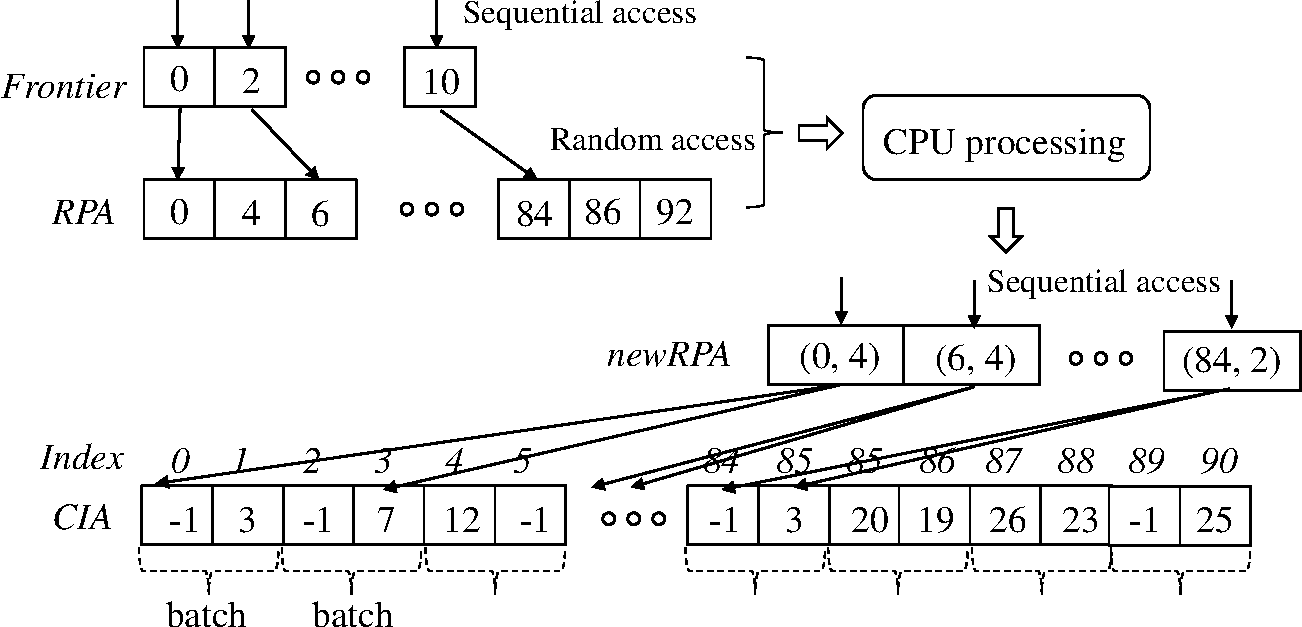
\includegraphics[width=0.85\linewidth]{reorg}}
%    \caption{RPA reorganization}
%\label{fig:reorg}
%\vspace{-1em}
%\end{figure}

\subsection{Level update shifting}
Since the level update i.e. $level[c\_out] \gets l + 1$ is essentially random 
write to DRAM, it is relatively slow and can affect the main BFS pipelining 
when it is put in the $inspectNgbVisitStatus()$. Nevertheless, we notice that
it does not affect the next BFS iteration thanks to the on-chip bitmap.
Particularly, the frontier vertices are already stored in memory in $updateFrontier()$, 
so we can always perform the level update based on just the stored frontier.
Therefore, we can safely shift level update processing out from 
the $checkNgbVisitStatus()$ and simplify the main BFS pipelining.
Meanwhile, we can postpone the level update without blocking the BFS processing.
With this observation, we propose a pipelining approach as shown in 
Figure \ref{fig:hyper}. Basically, we separate the level update from the 
main BFS pipeline and overlap it with the following BFS processing task, 
supposing there are continuous BFS tasks. While the level update is fast 
compared to the main BFS pipelining, it can either be processed on the 
attached host CPU or FPGA with lowest priority. 
\begin{figure}
	\center{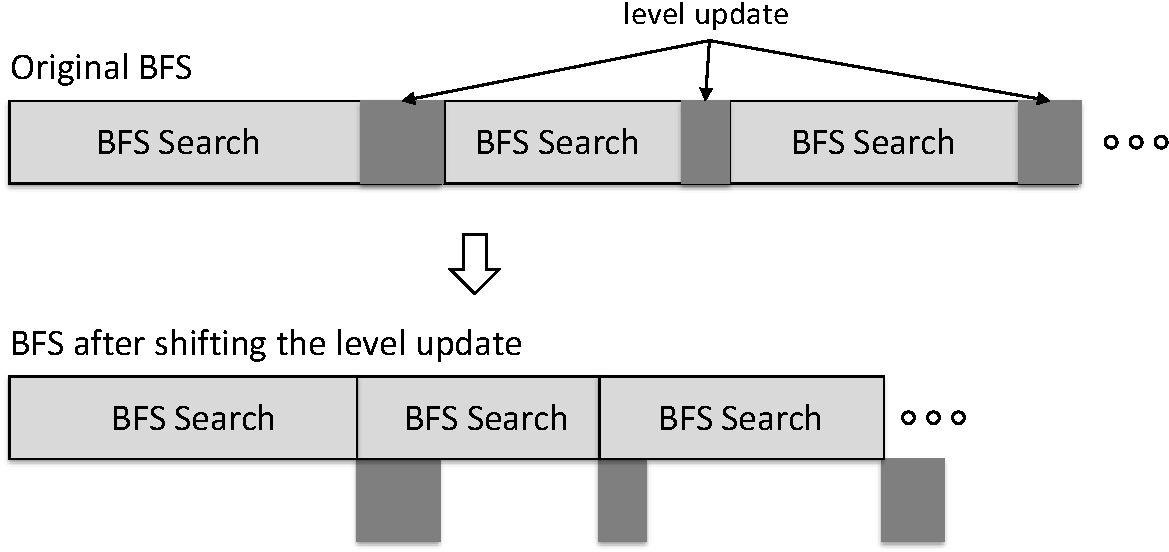
\includegraphics[width=0.7\linewidth]{hyper-pipeline}}
	\caption{Level update shifting with high-level pipelining}
\label{fig:hyper}
\vspace{-1.2em}
\end{figure}

%\subsection{Optimized BFS structure}
In summary, memory access is the performance bottleneck of BFS while the baseline 
BFS with OpenCL suffers rather low memory access efficiency. Targeting at 
the irregular BFS memory access patterns, we propose a series of optimizations to 
coalesce the memory accesses, reduce external memory accesses and shift the 
inefficient memory accesses from the main pipelining to improve the memory 
access efficiency, which ensures high-performance BFS on FPGAs with OpenCL.

%\begin{figure}
%	\center{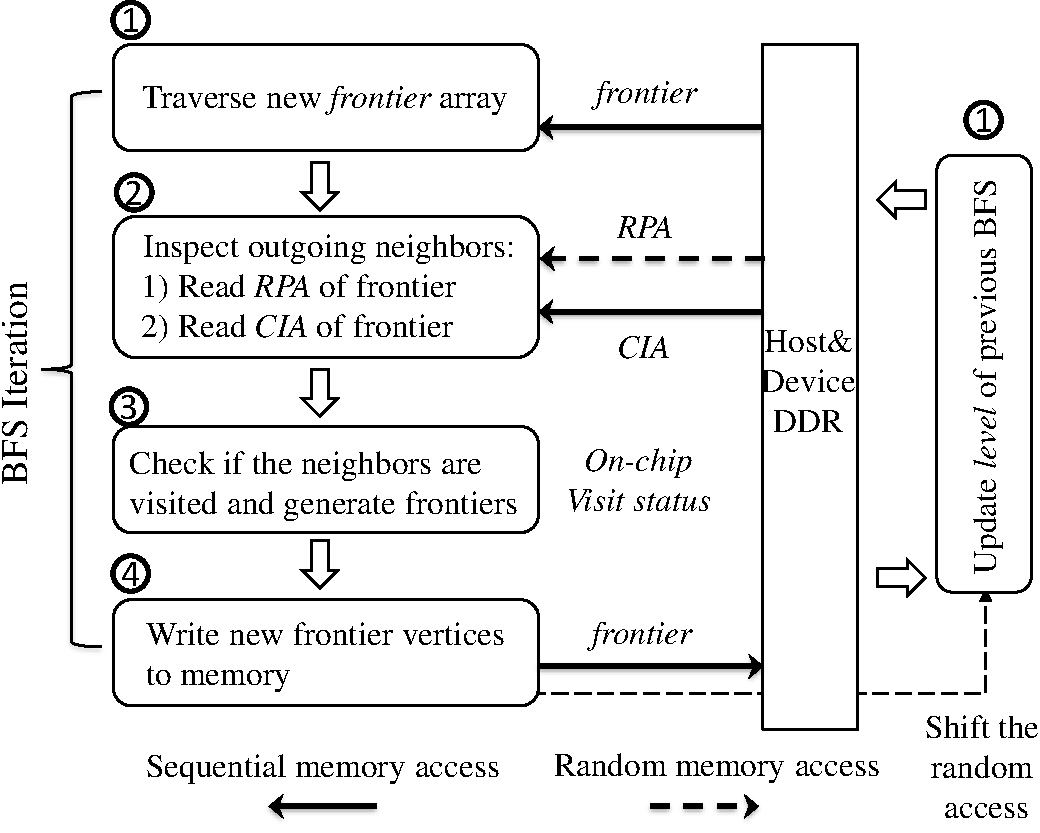
\includegraphics[width=0.75\linewidth]{opt-bfs}}
%    \caption{Optimized BFS pipeline}
%\label{fig:opt-bfs}
%\vspace{-1em}
%\end{figure}

